% Place after the open-loop trajectory-prediction table.
\begin{figure*}[t]
\centering
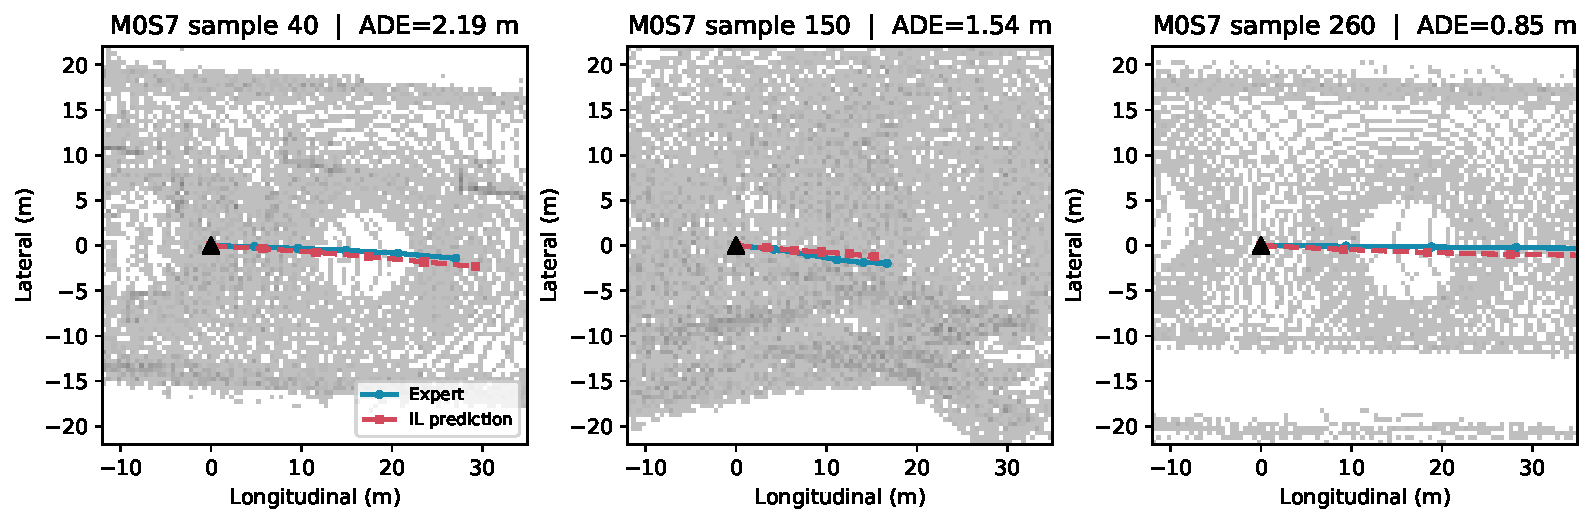
\includegraphics[width=0.96\textwidth]{figures/il_qualitative_m0s7.pdf}
\caption{Qualitative trajectory prediction on held-out M0S7 samples. The LiDAR BEV is shown in gray; blue and red denote the expert and imitation-policy trajectories, respectively.}
\label{fig:il_qualitative}
\end{figure*}

% Place after the action-conditioned boundary-risk results.
\begin{figure}[t]
\centering
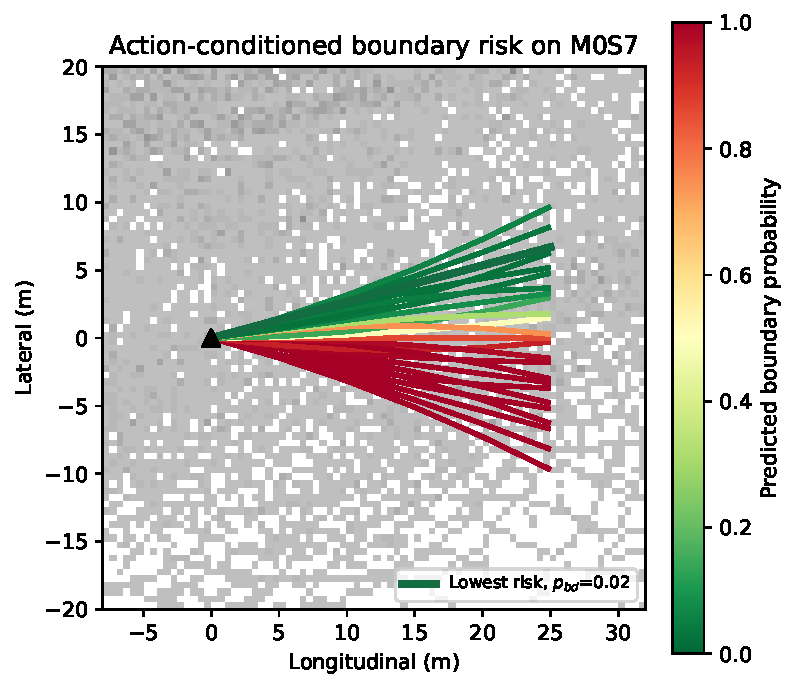
\includegraphics[width=0.95\columnwidth]{figures/boundary_candidate_screening.pdf}
\caption{Action-conditioned boundary-risk predictions for 25 candidate trajectories on M0S7. Color denotes predicted boundary probability, and the highlighted curve has the lowest predicted risk.}
\label{fig:boundary_candidates}
\end{figure}

% Place after the collision-prediction table.
\begin{figure}[t]
\centering
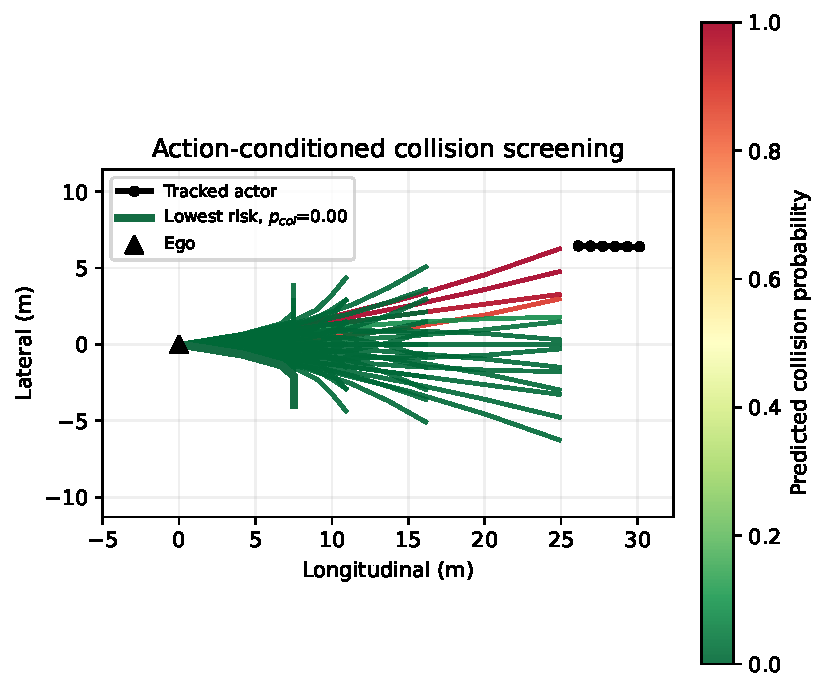
\includegraphics[width=0.95\columnwidth]{figures/collision_candidate_screening.pdf}
\caption{Collision-risk predictions for the 60 longitudinal and lateral candidates in a held-out replay interaction. The black trajectory denotes the tracked actor.}
\label{fig:collision_candidates}
\end{figure}

% Place after the dynamic-replay closed-loop table.
\begin{figure*}[t]
\centering
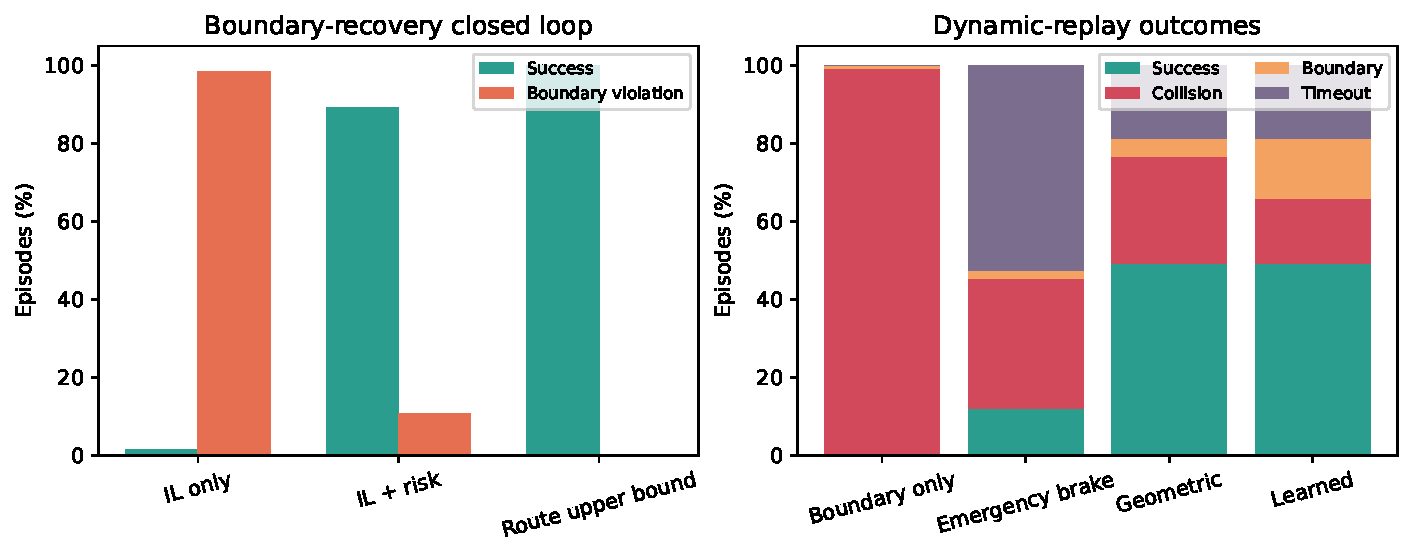
\includegraphics[width=0.92\textwidth]{figures/closed_loop_results.pdf}
\caption{Closed-loop outcomes on M0S7. Left: boundary recovery over 130 episodes. Right: outcomes for 150 controlled dynamic-replay interactions.}
\label{fig:closed_loop_results}
\end{figure*}
